% Diapositivas (Beamer) - Proyecto final MAT 4021 Matemáticas Discretas
% Compilar:  tectonic presentacion.tex      (o xelatex/lualatex)
\documentclass[aspectratio=169,11pt]{beamer}

\usetheme{metropolis}
\usepackage[spanish,es-noshorthands,es-tabla]{babel}
\usepackage{amsmath,amssymb}
\usepackage{booktabs}
\usepackage{tikz}
\usepackage{pgfplots}
\pgfplotsset{compat=1.18}
\usepackage[normalem]{ulem}

\definecolor{uninorte}{HTML}{C8102E}
\definecolor{oscuro}{HTML}{23373B}
\setbeamercolor{frametitle}{bg=oscuro,fg=white}
\setbeamercolor{progress bar}{fg=uninorte}
\setbeamercolor{alerted text}{fg=uninorte}
\metroset{numbering=fraction,progressbar=frametitle}

\newcommand{\repo}{\url{https://github.com/lau-240/Proyecto-final-Matem-ticas-Discretas}}

\title{Disponibilidad y uso de espacios del campus}
\subtitle{Álgebra booleana y grafos ponderados para encontrar un salón libre}
\author{\small Laura Vanessa Acuña Ordóñez \quad Isabella Barrios Pico \quad Ángel Gabriel Carrillo Henao\\
Montserrat Mariottis Martínez \quad Javier Enrique Torregrosa Lascano}
\institute{MAT 4021 Matemáticas Discretas -- Universidad del Norte\\[2pt]
\footnotesize\repo}
\date{Noviembre de 2026}

\begin{document}

\maketitle

% ------------------------------------------------------------------
\begin{frame}{El problema}
\begin{columns}[T]
\column{0.55\textwidth}
\begin{itemize}
  \item Buscar un salón libre para estudiar o reunirse = caminar de bloque en bloque.
  \item Los horarios de clase ocupan los salones solo en algunas franjas.
  \item No hay un lugar donde consultar la disponibilidad.
\end{itemize}
\column{0.42\textwidth}
\begin{block}{Dos preguntas}
\begin{enumerate}
  \item ¿Qué espacios están \alert{libres} en un intervalo?
  \item ¿Cuál queda \alert{más cerca} de mí?
\end{enumerate}
\end{block}
\end{columns}
\end{frame}

% ------------------------------------------------------------------
\begin{frame}{Idea: el problema ya es discreto}
\begin{columns}[T]
\column{0.48\textwidth}
\textbf{Álgebra booleana}
\begin{itemize}
  \item Tiempo en franjas de 1 hora.
  \item Horario $=$ subconjunto de franjas.
  \item Subconjunto $=$ vector de bits.
\end{itemize}
\column{0.48\textwidth}
\textbf{Grafos ponderados}
\begin{itemize}
  \item Bloques $=$ vértices.
  \item Caminos $=$ aristas con peso en minutos.
  \item Más cercano $=$ Dijkstra.
\end{itemize}
\end{columns}
\end{frame}

% ------------------------------------------------------------------
\begin{frame}{Franjas horarias como bits}
Lunes a sábado, 6:00 a 22:00 $\Rightarrow$ $6\times 16 = 96$ franjas.
\[
  f(d,h) = 16\,d + (h-6), \qquad \mathcal{F}=\{0,\dots,95\}
\]
Un conjunto $S\subseteq\mathcal{F}$ se guarda como el entero
$\chi(S)=\sum_{f\in S}2^f$.

\medskip
\begin{center}
\begin{tabular}{@{}lll@{}}
\toprule
Conjuntos & Bits & Uso en el modelo \\
\midrule
$S\cup T$ & \texttt{s | t} & agregar un uso \\
$S\cap T$ & \texttt{s \& t} & ¿se cruzan? \\
$\overline{S}$ & \texttt{\textasciitilde s \& U} & franjas no ocupadas \\
$S\subseteq T$ & \texttt{s \& t == s} & ¿hay información de toda la ventana? \\
\bottomrule
\end{tabular}
\end{center}
\small $(\mathcal{P}(\mathcal{F}),\cup,\cap,\overline{\phantom{x}})\cong(\{0,1\}^{96},\lor,\land,\lnot)$: cada operación es \alert{una} instrucción.
\end{frame}

% ------------------------------------------------------------------
\begin{frame}{Modelo de tres estados}
Por cada espacio $e$ se guardan dos vectores: $O_e$ (ocupado) e $I_e$ (conocido), con $O_e\subseteq I_e$.
\[
\text{estado}(e,f)=\begin{cases}
\text{\textcolor{uninorte}{ocupado}} & f\in O_e\\[2pt]
\text{\textcolor{teal}{libre}} & f\in I_e\setminus O_e\\[2pt]
\text{\textcolor{gray}{desconocido}} & f\notin I_e
\end{cases}
\]
\begin{alertblock}{Clave}
\emph{Sin información no significa libre.} Un modelo de dos estados supone que sí, y se equivoca.
\end{alertblock}
\end{frame}

% ------------------------------------------------------------------
\begin{frame}{Disponibilidad y conflictos}
Ventana pedida $W$ (ej.\ lunes 10:00--12:00):
\begin{itemize}
  \item \textbf{Disponible}: $O_e\cap W=\varnothing$ \ y \ $W\subseteq I_e$\\
  \hspace{1em}\texttt{(o \& w) == 0 and (i \& w) == w}
  \item \textbf{Conflicto al reservar}: $O_e\cap W\neq\varnothing$
  \item \textbf{Registrar}: $O_e\leftarrow O_e\cup W$, \ $I_e\leftarrow I_e\cup W$
\end{itemize}
\medskip
Costo $O(1)$: no depende de cuántas horas tenga $W$.

\medskip
\small Los usos de una sola vez (estudio, reunión) \alert{vencen}: al vencer se quitan de $O_e$
\emph{y} de $I_e$, porque haber estado ocupado una vez no prueba que quede libre.
\end{frame}

% ------------------------------------------------------------------
\begin{frame}{El campus como grafo ponderado}
\begin{columns}[c]
\column{0.58\textwidth}
\centering
\begin{tikzpicture}[
  v/.style={circle,draw,fill=oscuro!10,minimum size=6mm,inner sep=0pt,font=\footnotesize},
  lab/.style={font=\scriptsize,fill=white,inner sep=1pt}, scale=0.95]
  \foreach \n/\x in {A/0,B/1.2,C/2.4,D/3.6,E/4.8,F/6}
    \node[v] (\n) at (\x,0) {\n};
  \foreach \n/\x in {L/0,K/1.2,J/2.4,I/3.6,H/4.8,G/6}
    \node[v] (\n) at (\x,-2) {\n};
  \node[v] (M) at (0,-3.4) {M};
  \node[v,font=\tiny] (LAB) at (1.4,-3.4) {LAB};
  \draw (A)--node[lab]{2}(B); \draw (B)--node[lab]{2}(C);
  \draw (C)--node[lab]{3}(D); \draw (D)--node[lab]{2}(E);
  \draw (E)--node[lab]{2}(F); \draw (F)--node[lab]{3}(G);
  \draw (G)--node[lab]{2}(H); \draw (H)--node[lab]{2}(I);
  \draw (I)--node[lab]{3}(J); \draw (J)--node[lab]{2}(K);
  \draw (K)--node[lab]{2}(L); \draw (L)--node[lab]{6}(M);
  \draw (L)--node[lab]{3}(LAB);
  \draw (B) to[bend left=35] node[lab]{4} (E);
  \draw (C) to[bend left=35] node[lab]{5} (F);
  \draw (F)--node[lab]{5}(I);
  \draw (H) to[bend left=30] node[lab]{4} (K);
\end{tikzpicture}
\column{0.4\textwidth}
\begin{itemize}
  \item $|V|=14$ bloques, $|E|=17$.
  \item Peso $=$ minutos de caminata (valores de ejemplo).
  \item Cada espacio pertenece a un bloque.
\end{itemize}
\end{columns}
\end{frame}

% ------------------------------------------------------------------
\begin{frame}{Espacio libre más cercano}
\begin{enumerate}
  \item $d(s,\cdot)$ desde el bloque origen $s$ con \textbf{Dijkstra}: $O((|V|+|E|)\log|V|)$.
  \item Filtrar espacios disponibles en $W$ (operaciones de bits).
  \item Ordenar por $\bigl(d(s,\text{bloque}(e)),\ \text{id}(e)\bigr)$.
\end{enumerate}
\begin{block}{¿Dónde estoy? (ubicación inferida)}
Si el estudiante cargó su horario: bloque de la clase actual $\to$ si no, la última que
terminó $\to$ si no, la próxima. Sin horario, la elige a mano.
\end{block}
\end{frame}

% ------------------------------------------------------------------
\begin{frame}{La aplicación (Streamlit)}
\begin{columns}[c]
\column{0.58\textwidth}
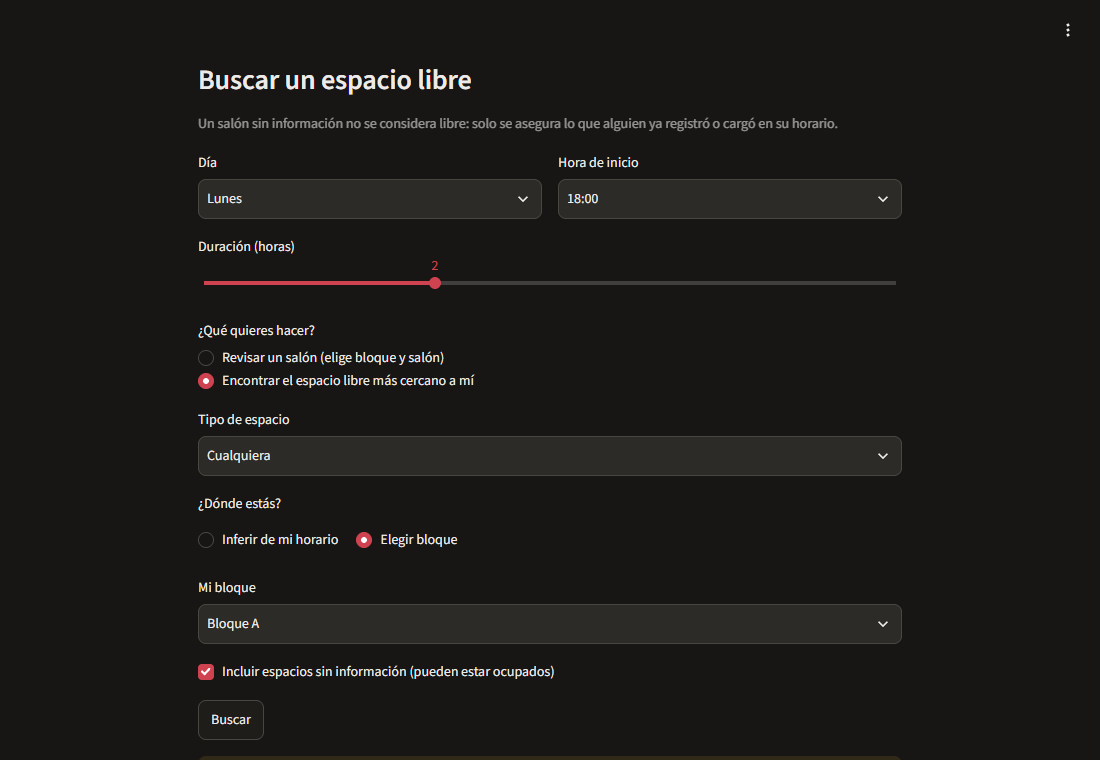
\includegraphics[width=\linewidth]{../figuras/app_buscar.png}
\column{0.4\textwidth}
\small
Pestañas:
\begin{itemize}
  \item Buscar libre / más cercano
  \item ¿Qué hay? (hora por hora)
  \item Tutorías
  \item Registrar y cargar horario (a mano o desde una foto con IA)
  \item Mi horario, Semestre
\end{itemize}
Código inventado, no nombre. Los datos vencen con el semestre.
\end{columns}
\end{frame}

% ------------------------------------------------------------------
\begin{frame}{Validación: caso de resultado conocido}
Campus pequeño: $A\overset{2}{-}B\overset{3}{-}C$. Lunes 10:00--12:00. Ana sale de clase en A1 a las 10:00.
\begin{center}
\begin{tabular}{@{}lll@{}}
\toprule
Salón & Estado 10--12 & \\
\midrule
A1 & ocupado (tutoría) & \\
A2 & desconocido & \\
B1 & libre, confirmado & a 2 min \\
C1 & libre, confirmado & a 5 min \\
\bottomrule
\end{tabular}
\end{center}
\begin{itemize}
  \item Solo confirmados $\Rightarrow$ \alert{B1 a 2 min} \checkmark
  \item Permitiendo desconocidos $\Rightarrow$ A2 a 0 min (marcado ``sin información'') \checkmark
  \item B1 14--16 y luego 15--17 $\Rightarrow$ conflicto ($W_1\cap W_2=\{15{:}00\}$) \checkmark
\end{itemize}
\small \textbf{104 pruebas} automáticas con \texttt{pytest} + GitHub Actions: todas pasan.
\end{frame}

% ------------------------------------------------------------------
\begin{frame}{Simulación: tres estados vs.\ dos estados}
\begin{columns}[c]
\column{0.55\textwidth}
\begin{tikzpicture}
\begin{axis}[width=\linewidth,height=5.2cm,
  xlabel={Cobertura de datos}, ylabel={Precisión de ``libre''},
  ymin=0.6,ymax=1.03,xmin=0.15,xmax=1,
  legend pos=south east, legend style={font=\scriptsize},
  tick label style={font=\scriptsize}, label style={font=\small},
  grid=major, grid style={gray!20}]
\addplot[mark=*,thick,color=teal] coordinates {(0.21,1)(0.41,1)(0.61,1)(0.80,1)(0.95,1)};
\addlegendentry{3 estados}
\addplot[mark=square*,thick,color=uninorte] coordinates {(0.21,0.67)(0.41,0.73)(0.61,0.80)(0.80,0.89)(0.95,0.98)};
\addlegendentry{ingenuo (2 estados)}
\end{axis}
\end{tikzpicture}
\column{0.42\textwidth}
\small
\begin{itemize}
  \item 42 espacios, ocupación aleatoria ($p=0{,}45$ por bloque de 2 h).
  \item Con 21\,\% de cobertura, el ingenuo falla en \alert{1 de cada 3} respuestas ``libre''.
  \item El 1,00 es por construcción: lo confirmado se supone correcto.
  \item Costo: con poca cobertura se encuentran menos espacios.
\end{itemize}
\end{columns}
\end{frame}

% ------------------------------------------------------------------
\begin{frame}{Análisis de la red del campus}
\begin{columns}[T]
\column{0.48\textwidth}
\textbf{Cercanía} $C(v)=\dfrac{|V|-1}{\sum_u d(u,v)}$
\begin{itemize}
  \item G, H: 0,137
  \item F: 0,134
\end{itemize}
\small Mejores lugares para servicios comunes.
\column{0.48\textwidth}
\textbf{Intermediación} $B(v)=\sum\limits_{s\neq v\neq t}\dfrac{\sigma_{st}(v)}{\sigma_{st}}$
\begin{itemize}
  \item F: 0,513
  \item G, H: 0,385
\end{itemize}
\small Bloques de paso: cerrar F alarga muchos recorridos.
\end{columns}
\end{frame}

% ------------------------------------------------------------------
\begin{frame}{Limitaciones y trabajo futuro}
\begin{itemize}
  \item Medir los tiempos reales de caminata (hoy son de ejemplo).
  \item Cargar horarios reales: la cobertura crece con el uso.
  \item El código estudiantil no es secreto; falta autenticación.
  \item JSON con candado sirve para un proceso; a escala, una base de datos.
  \item Encuesta: tiempo de búsqueda manual vs.\ con el modelo.
\end{itemize}
\end{frame}

% ------------------------------------------------------------------
\begin{frame}{Conclusiones}
\begin{itemize}
  \item Los horarios son conjuntos, y el álgebra booleana los vuelve operaciones de tiempo constante.
  \item Separar \emph{ocupado} de \emph{conocido} evita afirmar ``libre'' sin respaldo.
  \item Dijkstra convierte una lista de espacios libres en una recomendación.
  \item Las centralidades describen la estructura del campus.
\end{itemize}
\vfill
\begin{center}
\textbf{Código y README:}\\ \footnotesize\repo
\end{center}
\end{frame}

\begin{frame}[standout]
¡Gracias!\\[6pt]
\normalsize ¿Preguntas?
\end{frame}

\end{document}
